\chapter{Intelligent Data Acquisition Blends Targeted and Discovery Methods}

\section{Summary}

A MS method is described here that can reproducibly identify hundreds of peptides across multiple experiments. The method uses intelligent data acquisition (IDA) to precisely target peptides while simultaneously identifying thousands of other, non-targeted peptides in a single nano-LC-MS/MS experiment. We introduce an online peptide elution order alignment (EOA) algorithm that targets peptides based on their relative elution order, eliminating the need for retention time-based scheduling. We have applied this method to target 500 mouse peptides across six technical replicate nano-LC-MS/MS experiments and were able to identify 440 of these in all six, compared to only 201 peptides using data-dependent acquisition (DDA). A total of 3,757 other peptides were also identified within the same experiment, illustrating that this hybrid method does not eliminate the novel discovery advantages of DDA. The method was also tested on a set of mice in biological quadruplicate and increased the number of identified target peptides in all four mice by over 80\% (826 vs. 459) compared with the standard DDA method. We envision real-time data analysis as a powerful tool to improve the quality and reproducibility of proteomic datasets.

\section{Introduction}

Large-scale proteomic studies make use of a variety of tools and techniques to achieve depth and wide coverage of proteomes. The most popular method for sequencing proteomes is shotgun sequencing where peptides are digested from extracted proteins, separated with chromatography (HPLC), and then mass analyzed using mass spectrometry (MS).\cite{mudpit,mudpit2} Since complex proteomes can encompass thousands of proteins, leading to millions of peptides, deciding how to allocate the limited mass spectrometer bandwidth is key to successful analysis.\cite{100000} By far the most successful method for this time management is data dependent acquisition (DDA), where intact peptide precursors are first mass analyzed (MS), specific \mz{} features are then selected to undergo fragmentation, and finally the fragment ions are mass analyzed again (MS/MS). This process is repeated throughout the LC separation, resulting in a large collection of MS and MS/MS spectra. Peptides are eventually identified from the fragmentation spectra and then assembled together back into protein groups.\cite{sequest,sadygov,venable,panda,grouping} This approach has produced outstanding results in the past decade, but, due to variety of reasons (e.g., large protein dynamic range, speed of MS instrumentation, separation efficiency, etc.) undersampling of proteomes is very common. In other words, not every peptide is identified in every LC-MS/MS experiment. Incomplete datasets limit the questions researchers can answer; especially when biological replication is used to increase statistical power, many measurements become worthless if they cannot be measured reproducibly.\cite{quant} As proteomics seeks to answer global biological questions, reproducible peptide identification between datasets is mandated.\cite{ideker,msbp,molloy}

Many studies have outlined the problem of poor peptide reproducibility.\cite{liu,mrm,tabb,bigtime,pachl} Aebersold succinctly summarized that irreproducibility is a multifaceted issue, depending on user experience, equipment, and data analysis, among others.\cite{aebersold} He outlines that there are two main approaches in tackling irreproducibility. First, exhaustively identify every peptide in a sample---an approach that is becoming more feasible as technology improves.\cite{thakur,nagaraj,onehour} The more common approach, as many other researchers have embarked on, is to focus on a smaller subset of peptides and to thoroughly identify and quantify those using targeted methods.\cite{savitski} Methods such as selected reaction monitoring (SRM) are powerful and reproducible, but are low throughput, targeting a few hundred peptides at most.\cite{lange,picotti1,picotti2,picotti3,bigsrm} To improve identification reproducibility and throughput, targeted methods almost exclusively rely on retention time-based scheduling, segmenting the MS duty cycle among the target peptides. In SRM methods, a series of MS/MS transitions for each targeted peptide is automatically collected at the appropriate retention time (RT), removing the dependence on MS detection. This requires precise knowledge of the peptide retention time for the LC-MS system and is low throughput as only one set of transitions are monitored at a given point in time. Recent work on intelligent SRM (iSRM) increases throughput by monitoring only a subset of transitions for each target, switching to normal SRM when these transitions are detected.\cite{isrm} We sought to expand upon the idea of intelligent real-time switching of methods by combining the enhanced reproducibility of targeted scheduled methods with the novel discovery advantages of DDA in a single hybrid method. Our goals were three-fold: first, to develop a method that increases the throughput of targeting; second, to replace retention-time based scheduling and its laborious method development with a more robust and straightforward peptide elution ordering; and last, to maintain the discovery aspect of DDA sampling while simultaneously targeting a subset of peptides.

In the last decade, a few computational approaches have been aimed at solving the problem of poor reproducibility. The concept of accurate mass tags (AMT) was first introduced by Smith et. al. as a means to identify peptides in multiple runs based on accurate mass and retention time.\cite{smith} This concept was further expanded with PepMiner and PEPPeR, tools for clustering features among multiple datasets.\cite{pepminer,pepper} Most notably, Prakash et. al. introduce the concept of aligning multiple MS datasets based on peptide relative elution order into signal maps.\cite{prakash} To date, these and other computational methods\cite{radulovic,listgarten,shen,zhang,lin,bateman} have been performed post-acquisition, attempting to improve already collected data. We seek to improve the reproducibility at the source by improving the algorithms the MS uses to select precursors to fragment. We and others have proposed using real-time data analysis and dynamic MS control as a means for improving the quality of acquired spectra.\cite{inseq,graumann,webber} Here we present our findings on combining accurate mass, elution orders, and real-time data analysis to improve the sampling reproducibility of the MS.

\section{Results and Discussion}

\subsection*{Irreproducible Peptide Identification.}
In data dependent acquisition (DDA) peptide precursors are selected for fragmentation based on intensity in a MS survey scan. This straightforward approach has proven to be a simple and powerful technique. However, it is pestered with inconsistent sampling, and therefore, irregular peptide identification between experiments. The DDA method is inherently stochastic in nature, depending heavily on the consistency of the input data (MS) to deliver reproducible peptide identification (MS/MS). Even the slightest change in the chromatography or ionization efficiencies will have repercussions on the collection of the whole dataset (e.g., the butterfly effect). To characterize the extent these minor changes have on the reproducibility of peptide identifications, six replicate injections of a tryptic digest of yeast whole cell lysate were analyzed using DDA on the same nano-LC-MS/MS system over a span of ten days. On average, each experiment identified 13,289 $\pm$340 unique peptide sequences (I/L ambiguity removed) at a 1\% FDR, indicating a highly consistent separation and nearly identical instrument performance. Of the 23,919 unique peptides identified in total, only 5,404 (22.6\%) of those peptide were identified in all six experiments (Figure \ref{fig:eoa1}).
\begin{sidewaysfigure}[p]
	\centering
	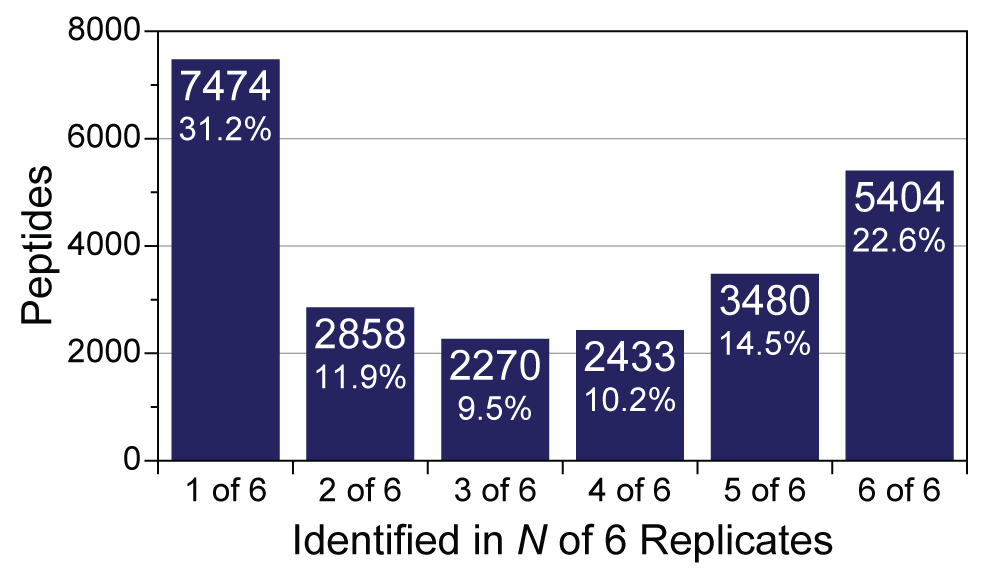
\includegraphics[width=\columnwidth]{eoa/EOA 1.png}
	\mycaption{Overlap of peptide identification among the analysis of six technical replicates}{Six nano-LC-MS/MS experiments produced 23,919 unique peptide identifications in total, but only one fifth of the identifications were observed in all six replicates. A large percentage (31.2\%) of the peptides were only detected in one of the six experiments.}
	\label{fig:eoa1}
\end{sidewaysfigure}
A significant portion were only identified once (7,474 31.2\%) while the remaining peptides were divided between two and five experiments. This clearly demonstrates the irreproducibility of DDA sampling on the same peptide solution. The reproducibility of identified protein groups fares better; 1,708 of 3,054 (56\%) protein groups were identified in every experiment. The higher overlap percentage is because many different peptides can make up one protein group, minimizing the importance of identifying the same peptides in all experiments. However, post translational modification (PTM) analysis requires identification of the same sites to compare between experiments, demanding the need for high peptide overlap. PTM analysis and quantitation is becoming more prominent in the literature, thus making this a growing problem in the field. Two reasons can be attributed to the poor reproducibility of stochastic DDA sampling. First, precursors having low signal-to-noise (S/N) are affected first by changes in chromatography and ionization. For example, a precursor with a maximal S/N of 4 may have been sampled and identified in one experiment, but in the next experiment the S/N may have dropped below the detection threshold and excluded from being sampled. This is evident when 8,883 MS features from peptides identified in one or all of the six experiments were examined for their maximal S/N (Figure \ref{fig:eoas1}).
 \begin{sidewaysfigure}[p]
 	\centering
 	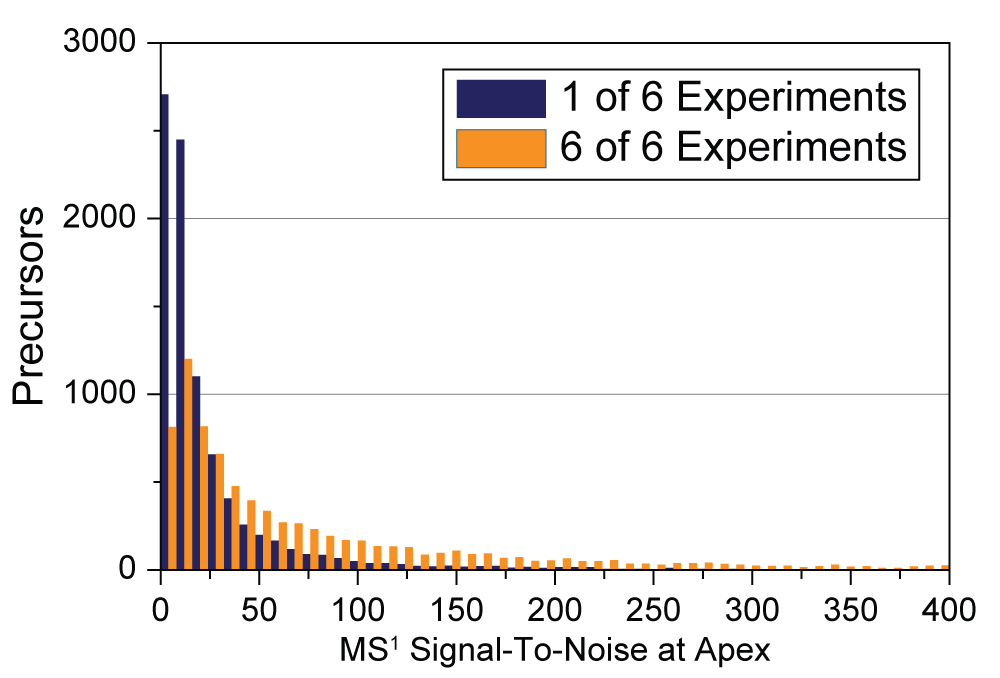
\includegraphics[width=0.9\columnwidth]{eoa/EOA S1.png}
 	\mycaption{Distribution of signal-to-noise ratios of reproducible and irrepoducible peptide identifications}{Peptides that were identified in 1 of 6 or 6 of 6 DDA top-15 experiments were analyzed for their maximal MS signal-to-noise (S/N). A larger percentage of those peptides seen only once appear at lower signal-to-noise values, indicating that MS signal intensity for reproducible identifications.}
 	\label{fig:eoas1}
 \end{sidewaysfigure}
For peptides identified once 2,707 (30.5\%) had a maximal S/N $\leq$ 4 while only 814 (9.2\%) precursors identified in every experiment had similar maximum S/N. The other reason for inconsistent peptide identification is increased MS spectral complexity, specifically its effect on charge-state assignment. In proteomic MS/MS workflows, precursors are often only selected when they exhibit a well-defined charge state---usually where \textit{z} > 1, as singly charged precursors fragment poorly and usually do not lead to positive identifications. Increases in spectral complexity hinder the charge-state determination algorithms, especially for low S/N precursors. This results in skipping precursors even if its signal-to-noise is above the sampling threshold.

\subsection{Retention Time Based Targeting.}

When good peptide identification reproducibility is needed, retention time (RT) based targeting, i.e., scheduling, has been the method of choice. Here, peptides of interest are assigned an expected elution time and MS/MS are triggered, regardless of MS detection, during the appropriate time range. This avoids the two issues with DDA sampling described above and enables much higher reproducibility. However, such methods are laborious to construct and maintain; identical LC and MS parameters must be kept between experiments to minimize any variances in retention times of the peptides.

To assess the degree of variance in peptide retention times that occur in normal nano-LC-MS/MS experiments, two of the yeast DDA experiments described above, performed ten days apart, were compared. The first experiment (July $22^{nd}$, D0) produced 13,529 unique peptides and the second experiment (July $31^{st}$, D9) identified 13,433 yeast peptides. Together, 7,589 peptides were in common and the apex of their retention time in each experiment is plotted in Figure \ref{fig:eoa2}A.
\begin{figure}[p]
	\centering
	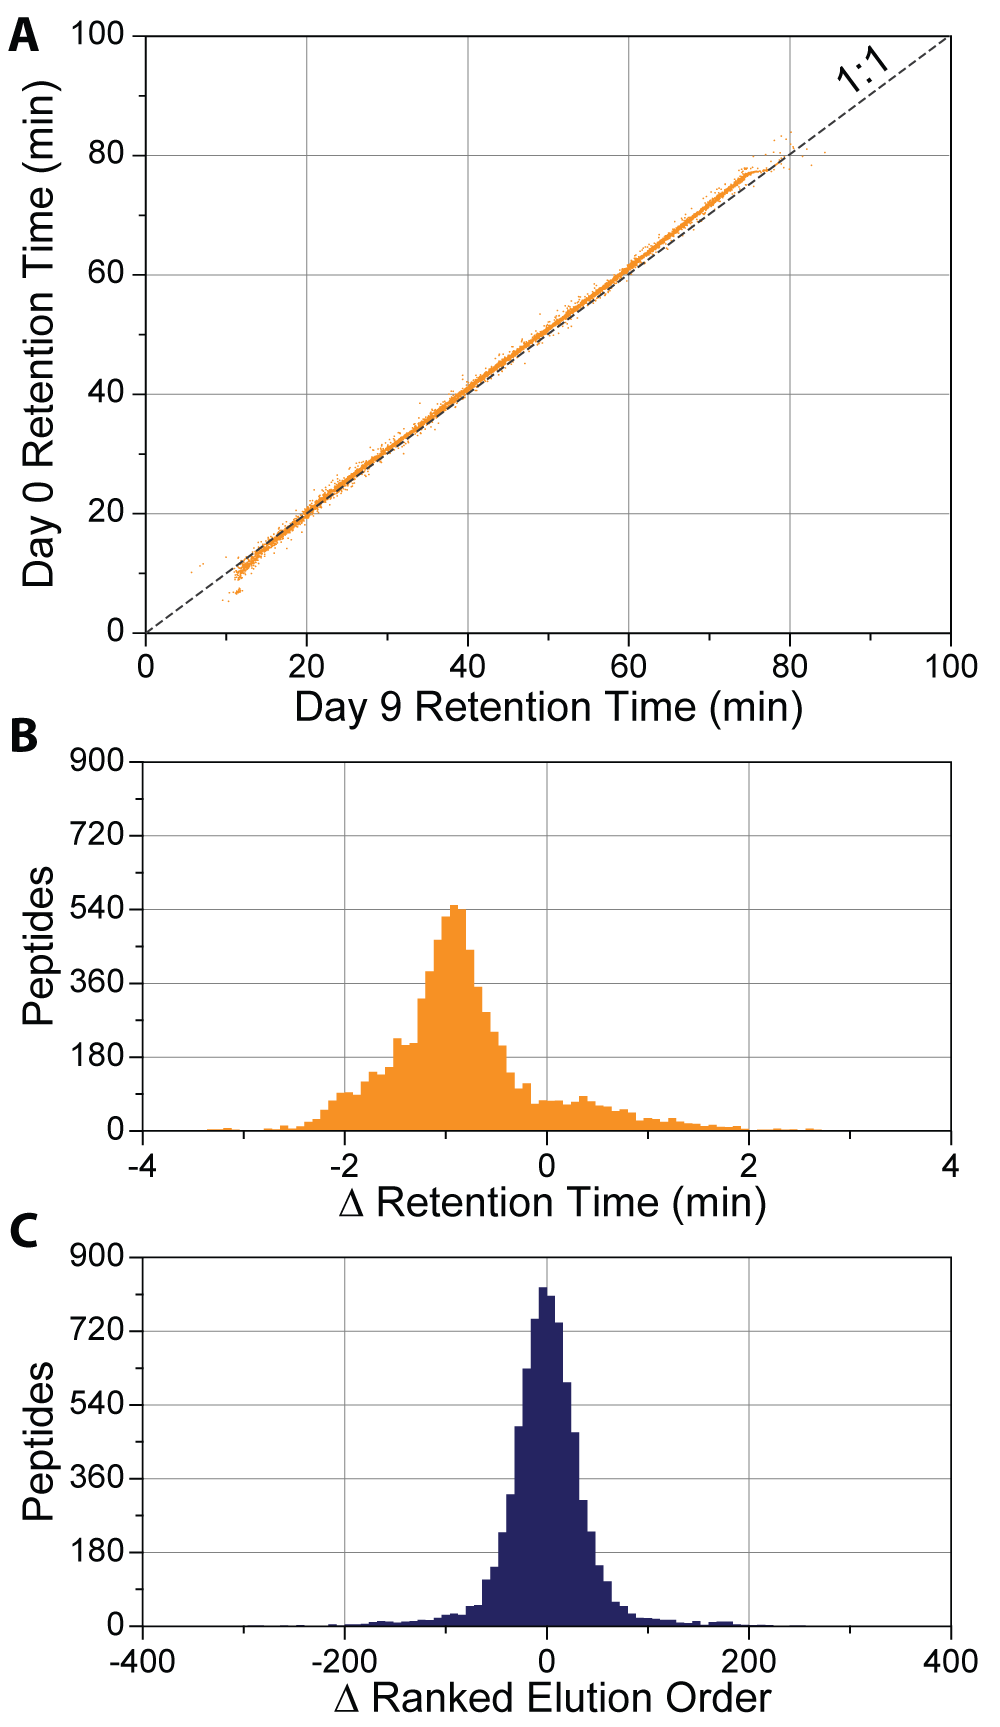
\includegraphics[width=0.65\columnwidth]{eoa/EOA 2.png}
	\mycaption{Retention time deviation between matched LC-MS/MS experiments}{To assess the deviation in retention times for matched samples two identical nano-LC-MS/MS experiments were run ten days apart on the same LC-MS system. (A) The relationship between apex retention times of the 7,589 unique peptides common between experiments display a high degree of linearity ($R^2$ = 0.9989) but a skewed slope and non-zero intercept (m = 1.033; b = -0.647).  (B) The average deviation from unity was nearly a minute off ($\mu$ = -0.805 min), with a broad distribution over 2 minutes wide. (C) Peptides ranked by their relative elution order exhibit a normal distribution around zero ($\mu$ =-1.097).}
	\label{fig:eoa2}
\end{figure} 

The relationship between retention times of matched peptides is highly linear ($R^2$ = 0.9989) but has a non-unity slope and non-zero intercept (m = 1.033; b = -0.647). While the slope is very close to 1, even the slightest deviation (0.033), compounded over time, leads to large RT differences late in the separation (e.g., \textasciitilde1.6 min shift at 70 min). On the whole, the average RT deviation was nearly a minute ($\mu$ = -0.805 min) with a broad distribution over a two minute range (Figure \ref{fig:eoa2}B). Typically, the assigned peptide elution times must be corrected to encompass this shift.

We hypothesize that---due to the degree of linearity in peptide retention times,we could avoid these corrections by scheduling peptides based on their relative elution order (EO), opposed to their absolute retention time. Under similar LC conditions (i.e., same particles, temperature, column length, phase, etc.) peptides elute in the same relative order regardless of separation duration or slope. For example, if peptide 'A' elutes before peptide 'B' in a 30 minute LC gradient, the same ordering is preserved with a 60 minute LC gradient, even if the absolute retention times vary greatly. When many peptides' elution orders are taken into account (e.g., 1000s of peptides) they provide a simple way to correct for elution variation dynamically. This is evident when we took the 7,589 peptides and rank ordered them based on their apex retention times for both the D0 and D9 experiments and plotted the difference between matched peptides (Figure \ref{fig:eoa2}C). Here the values are normally distributed around zero ($\mu$ =-1.097) with a full width at half maximum (FWHM) of only \textasciitilde100.
\begin{figure}[p]
	\centering
	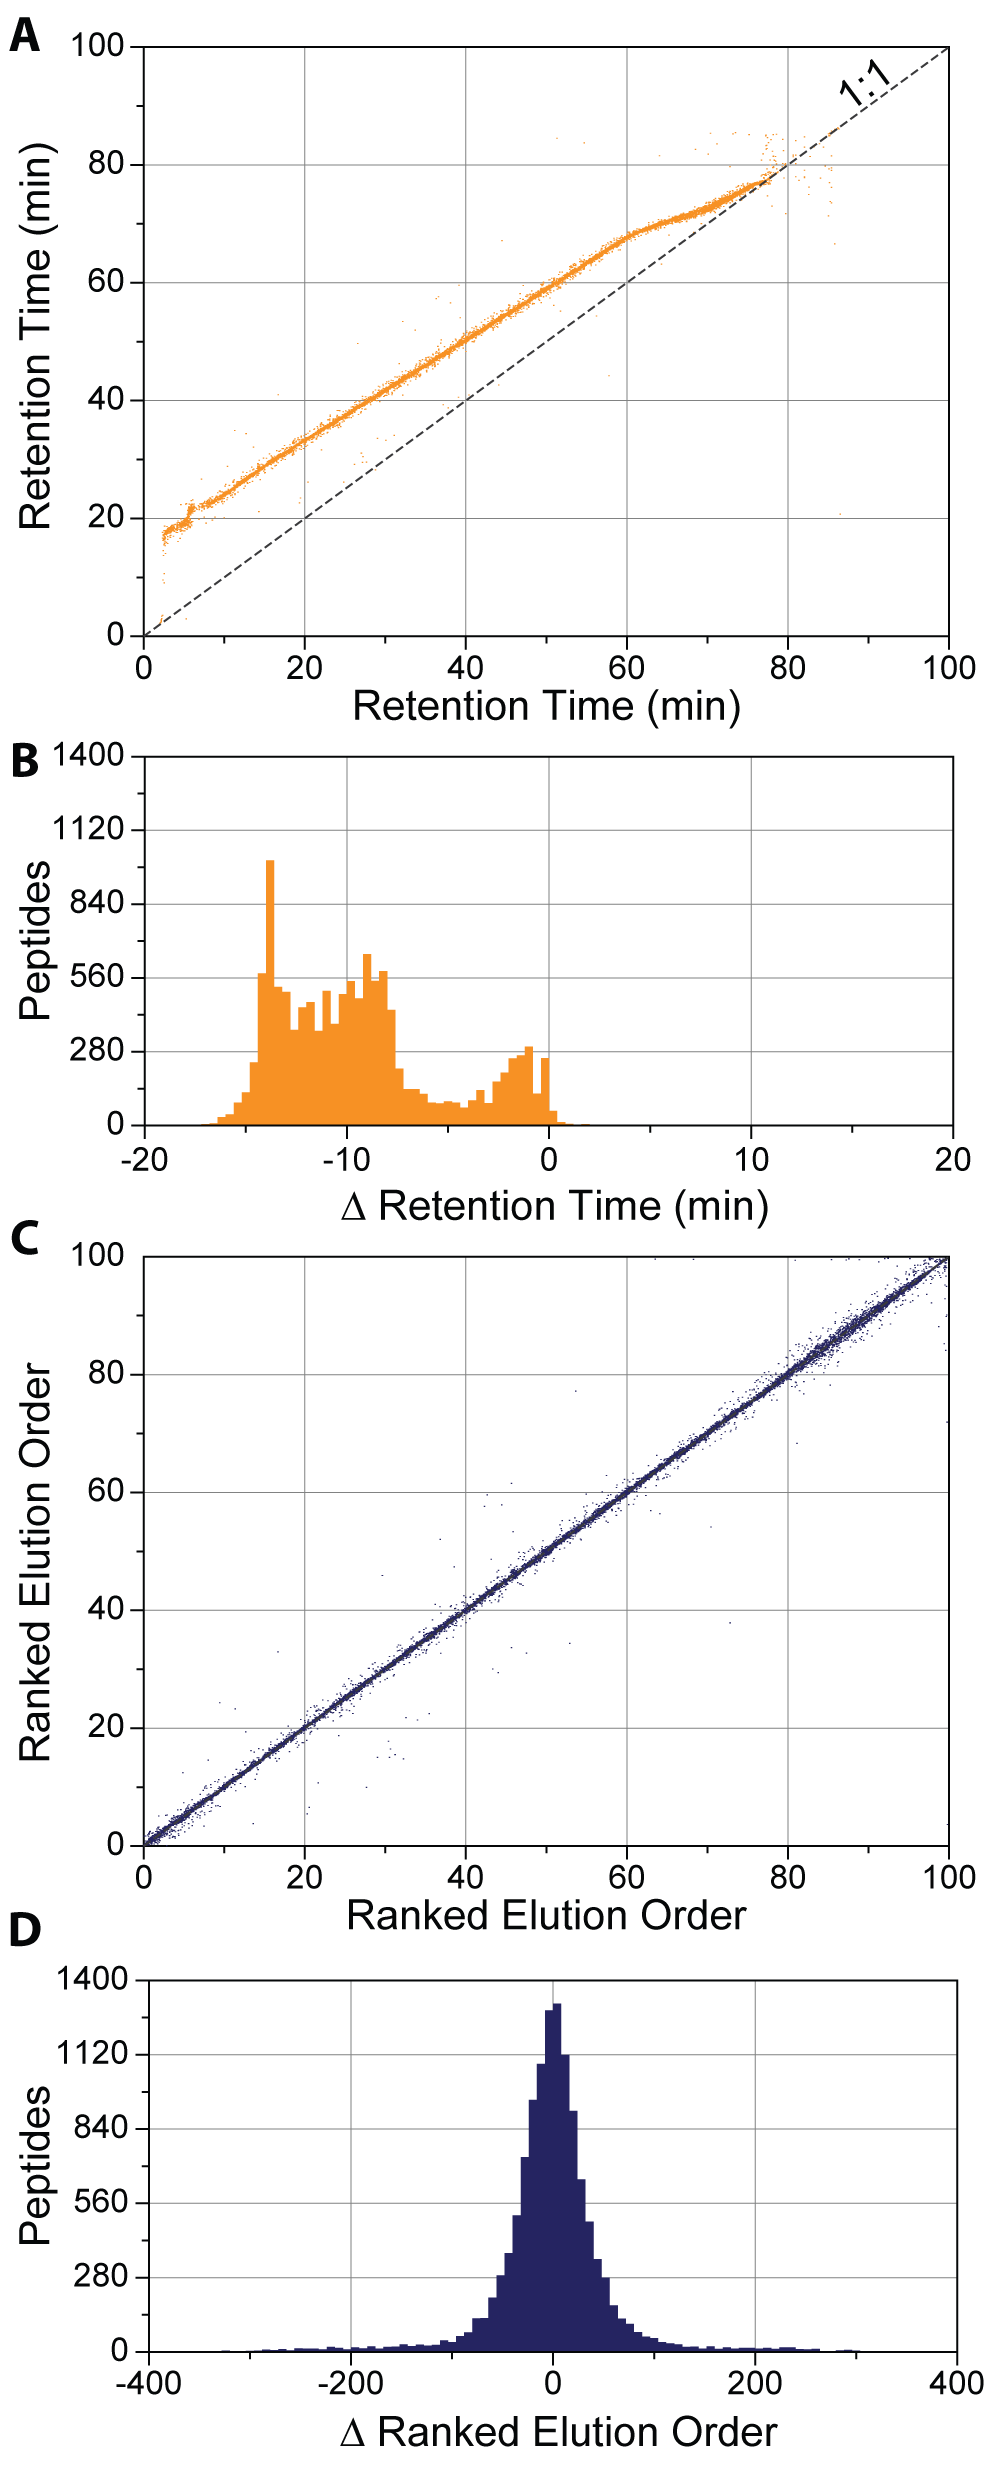
\includegraphics[width=0.5\columnwidth]{eoa/EOA S2.png}
	\mycaption{Two technical replicates of a yeast DDA top-15 method using two different LC gradients}{(A) Retention times for matched peptides between the two gradients is linear but not 1:1. (B) An average deviation of 10 min exists between the two experiments. (C) Rank elution orderings of matched peptides between the two gradients show a highly linear relationship that is exactly 1:1. (D) The average deviation in elution order for matched peptides is symmetric around 0.}
	\label{fig:eoas2}	
\end{figure} 

Elution order can be useful even under extreme differences in chromatographic conditions as well. To simulate dynamic chromatographic conditions, we separated yeast peptides under two different LC gradient profiles. The resulting peptide identifications were again matched between the runs and the retention time difference was plotted (Figure \ref{fig:eoas2}A). These data show an average deviation of ten minutes between the two gradients (Figure \ref{fig:eoas2}B), but when ranked by their elution orders, the two experiments show a linear slope of 1 with a normal distribution of ranked elution orders around zero (Figure \ref{fig:eoas2}C\&D). 

\subsection*{Real-time Elution Ordering Alignment.}

We reasoned that using elution order could improve the irreproducible sampling of DDA---similarly to scheduled methods, but on a larger scale and more robustly. The question shifts from ''What retention time is it?'' as scheduled methods ask, to ''What is the current elution order?'' By knowing which peptides are currently eluting from the LC, combined with the \emph{a priori} knowledge of their elution order, we predict with high fidelity which peptides are going to subsequently elute. 

Prior knowledge is needed of the sample to adequately calculate the elution orders of the peptides in the sample. With time-based scheduled methods, many cursory experiments are performed to optimize the retention times of the targeted peptides. To reduce variances in retention times, it's vital that these initial experiments are conducted exactly the same as the targeted experiments. In stark contrast, elution orders can be determined using a variety of methods. First, much work has been devoted to determining peptide hydrophobicities from theoretical calculations of the amino acid sequence.\cite{ssrcalc,ssrcalc2,petritis,spicer} A simple list of peptides, ordered by their hydrophobicities, can produce a highly linear elution ordering. Second, previously collected data of the sample can produce an accurate elution ordering as long as the LC conditions are similar enough. This enables the combination of multiple datasets to produce a single elution order vs. \mz{} map (elution order map, EOM), regardless of their individual separation durations. This is accomplished by rank ordering all the peptide identifications in a given run and normalizing their orderings between 0 and 100 (where 100 represents the last eluting peptide). These normalized values are then matched between experiments and aligned using a simple algorithm to produce the final EOM as shown in Figure \ref{fig:eoa3}A.
\begin{sidewaysfigure}[p]
	\centering
	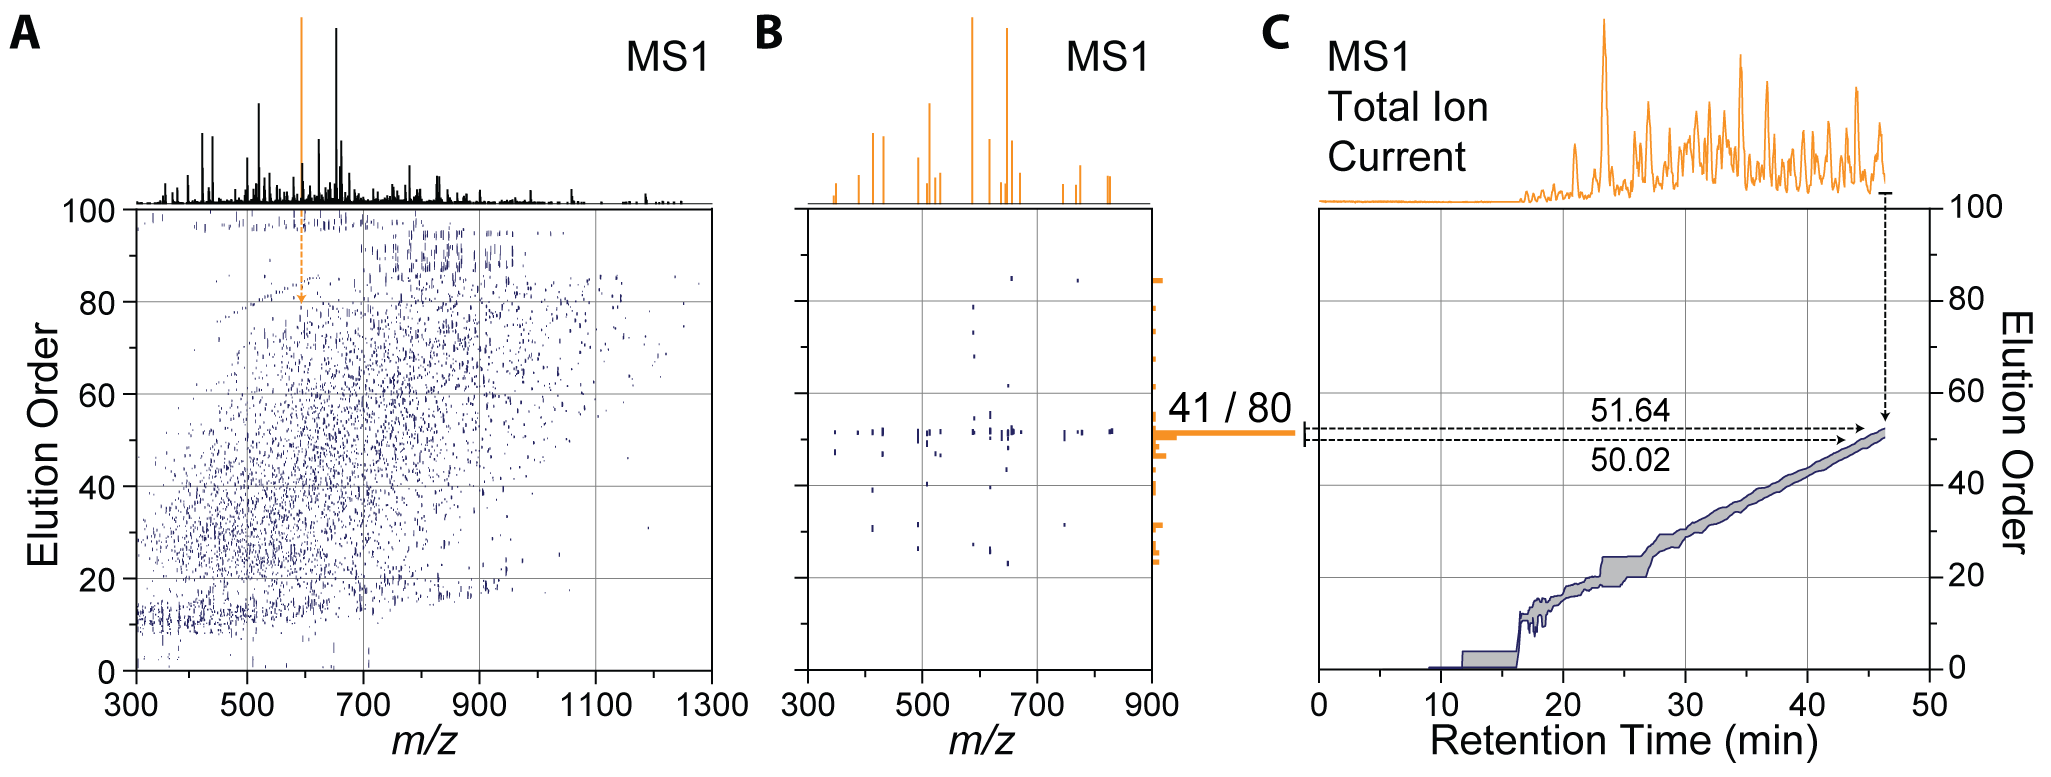
\includegraphics[width=\columnwidth]{eoa/EOA 3.png}
	\mycaption{Real-time elution order alignment algorithm}{After 46.3 minutes into a LC-MS/MS experiment, an MS scan is performed (A) and \mz{} features are matched to a 2D ion map stored on the instrument. (B) 21 of the peaks match 80 features in the ion map at a 10 ppm tolerance. Of these, over half (41 of 80) were mapped to one elution order bin (51 elution order). (C) A rolling elution order range is continually updated throughout the LC-MS/MS experiment.}
	\label{fig:eoa3}
\end{sidewaysfigure}
Lastly, the most robust method for determining peptide elution orders is to perform a discovery experiment right before the targeted experiment. Regardless of how elution order is determined, the final EOM is uploaded onto the instrument and is accessed throughout the course of the subsequent analyses.

Prior to targeted analysis, a list of peptide targets, along with their relative elution orders are also uploaded to the instrument (Figure \ref{fig:eoa4}B).
\begin{sidewaysfigure}[p]
	\centering
	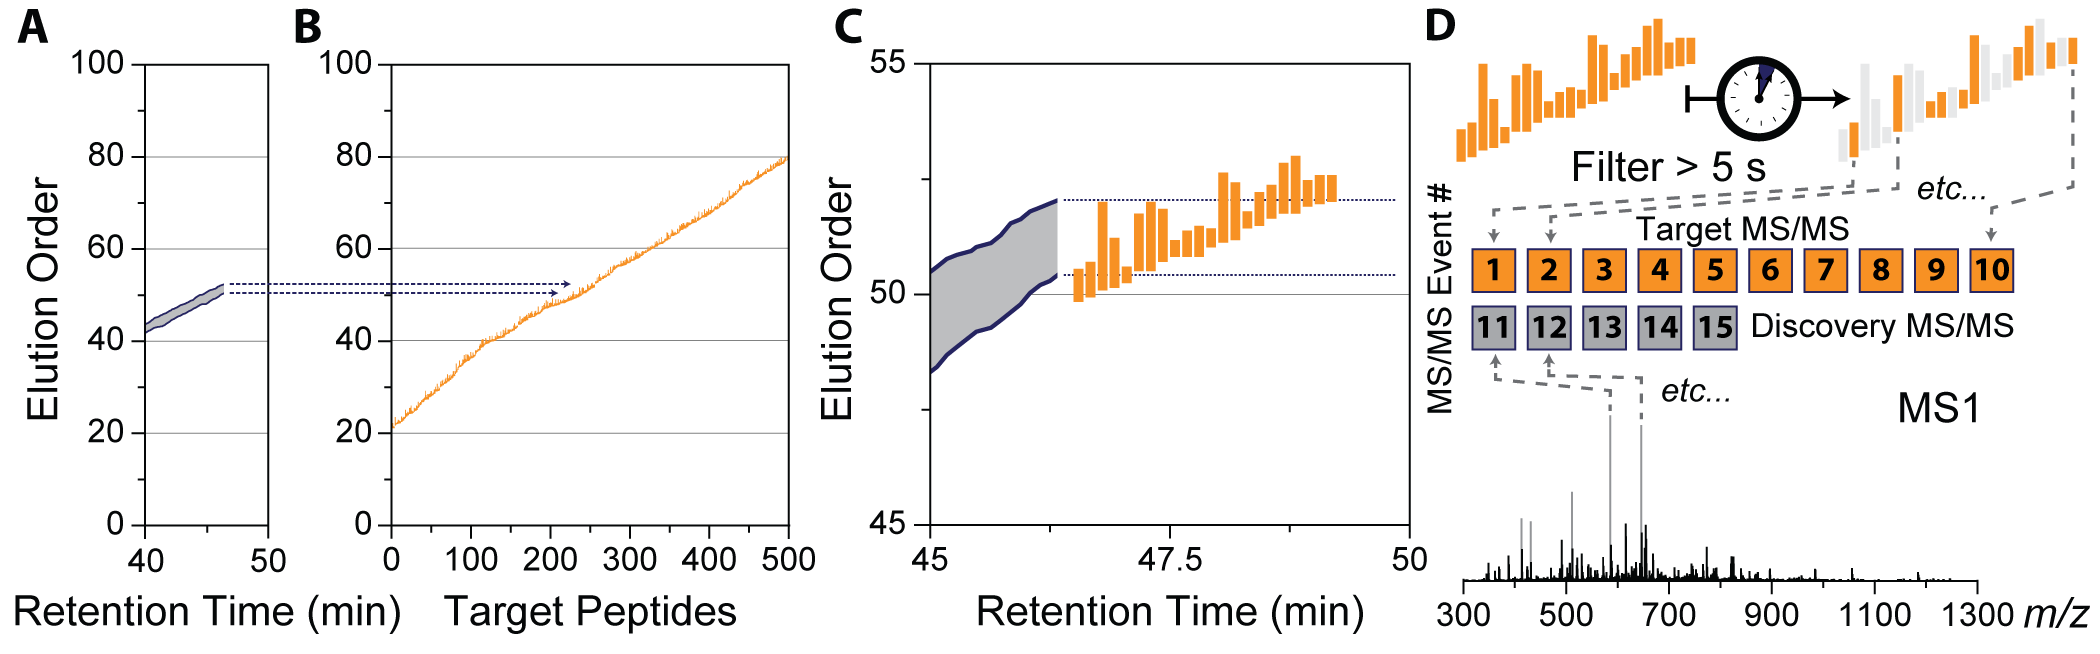
\includegraphics[width=\columnwidth]{eoa/EOA 4.png}
	\mycaption{Selection of targets within elution order range}{Following determination of the current elution order range (A), targets sharing a similar elution order are selected (C). Peptide targets within the elution order range are sorted based on when they were last sampled for MS/MS, leaving targets that have been waiting the longest. Those peptides are immediately sampled, regardless of MS detection (D). Remaining MS/MS events are automatically filled with DDA chosen \mz{} features.}
	\label{fig:eoa4}
\end{sidewaysfigure} 
Each target is assigned an elution order range depending on how long it was identified in the discovery experiments (see Figure \ref{fig:eoa4}C for zoom in). During the targeted analysis, instead of relying on absolute retention time to trigger targeted MS/MS, determining the current elution order becomes the main goal of the method. We have designed an online peptide elution order alignment (EOA) algorithm that takes a single MS spectrum and computes the current elution order therefrom. In brief, following MS acquisition, the EOA algorithm takes the most intense \mz{} feature and extracts all the elution order values from the uploaded EOM at a narrow \mz{} tolerance (e.g., 10 ppm) (Figure \ref{fig:eoa3}A). Each \mz{} feature is matched in a similar fashion and the resulting EO values are stored in a separate array (Figure 3B). In this example MS, 21 \mz{} features matched a total of 80 EO values. When analyzed, 41 of these values are contained within a single 1 EO-wide bin. This indicates with high confidence that the current elution order is near this maximum. To determine the elution order precisely, the algorithm then calculates the 95\% confidence interval around the max EO bin and stores the minimum (50.02) and maximum (51.64) elution order. This process is repeated for each MS and over time the calculated elution order range constructs a rolling-average as shown in Figure 3C. The EOA algorithm is expedient, taking on average 26 ms per MS to execute and does not induce a statistically significant change in the total number of MS/MS scans performed (Figure \ref{fig:eoas3}).
\begin{figure}[p]
	\centering
	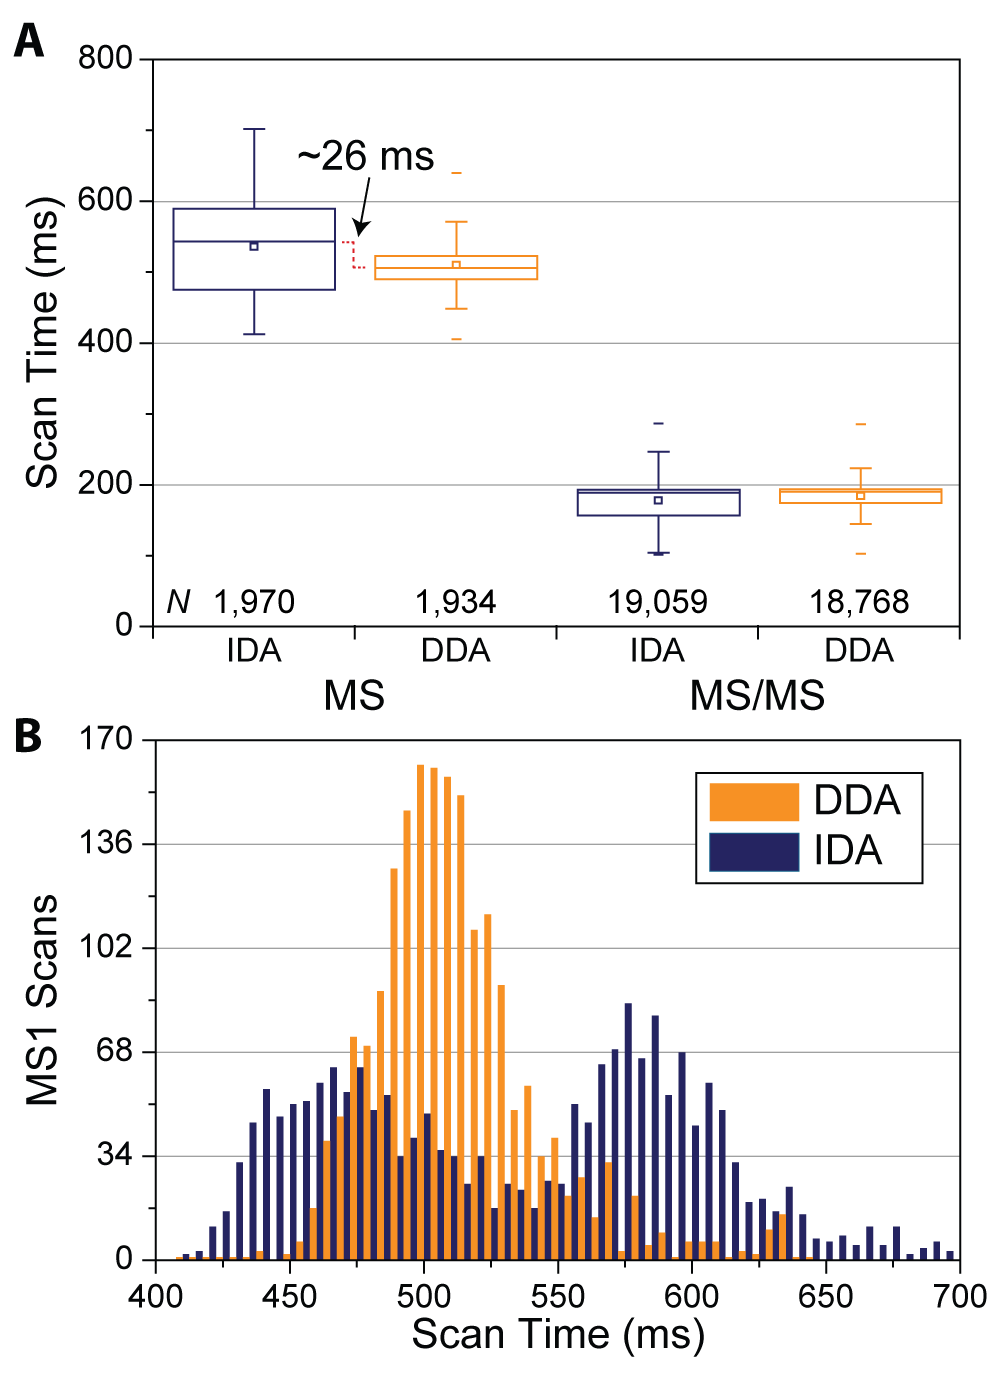
\includegraphics[width=0.8\columnwidth]{eoa/EOA S3.png}
	\mycaption{Duty cycle of elution order alignment algorithm}{(A) The elution order alignment (EOA) algorithm is expedient and induces only a slight increase in the MS duty cycle compared to normal DDA method (\textasciitilde26 ms). (B) The distributions of scan times for IDA is bimodal because the EOA algorithm can be triggered every other MS, because the current elution order changes only slightly between consecutive MS scans.}
	\label{fig:eoas3}
\end{figure} 

Once the current elution order range is determined, peptides sharing a similar elution order are selected for MS/MS analysis. Briefly, the current elution order range is intersected with the target peptides already uploaded on the instrument (Figure \ref{fig:eoa4}B) and overlapping peptides are stored as potential targets (Figure \ref{fig:eoa4}C). These peptides have a high probability of eluting next since they share very similar EO values with the current overall EO value. Since there can be many potential targets at any given time, they are filtered based on how long since they were last sampled, this is to prevent oversampling of any one target. Peptides that have been waiting the longest (i.e., > 5s) are automatically triggered for MS/MS analysis regardless of MS detection. Unfilled MS/MS events are then populated using normal DDA top-N approaches, excluding any \mz{} previously selected to be targeted (Figure \ref{fig:eoa4}D). This data collection scheme enables repetitive, consistent targeting of multiple peptides over their elution, while allowing DDA scans to facilitate discovery. The EOA algorithm is compatible with other quantitative strategies such as parallel reaction monitoring (PRM) where peptide targets are repeatedly sampled (MS/MS) over their elution, and the resulting fragment ions are extracted to provide quantitative information (Figure \ref{fig:eoas4}).\cite{prm,gallien}
\begin{figure}[p]
	\centering
	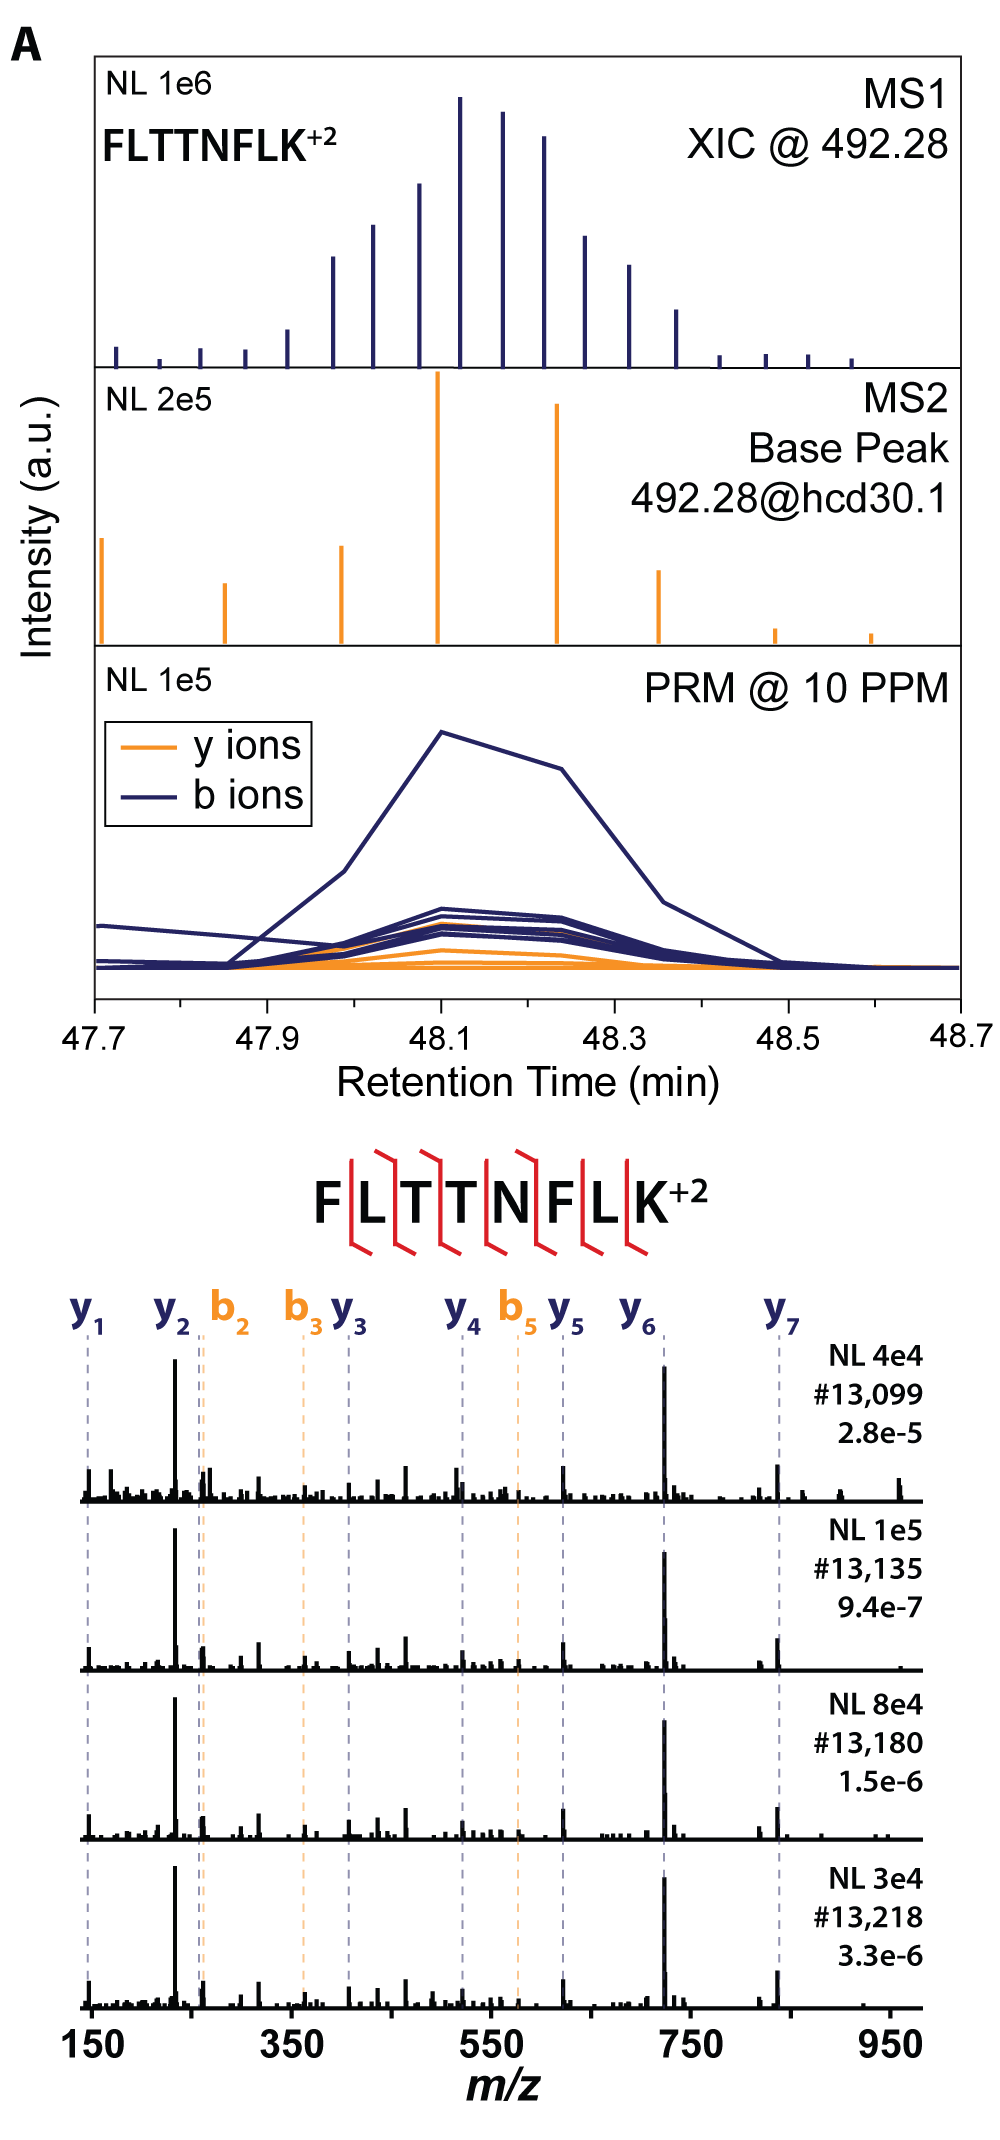
\includegraphics[width=0.6\columnwidth]{eoa/EOA S4.png}
	\mycaption{Parallel reaction monitoring (PRM) scan sequences obtainable using the IDA method}{(A) The peptide FLTTNFLK was MS/MS sampled approximately every 6 seconds over its elution profile. The b- and y-ions intensities were tracked over time to provide quantitative results.}
	\label{fig:eoas4}
\end{figure}  

\subsection*{Improving Peptide Identification in Multiple Experiments.}

We reasoned that the EOA algorithm would improve the reproducibility of peptide identification across multiple runs. Additionally, we increased the proteomic complexity by using a mammalian system (mouse) to determine how complexity affects the algorithm. To test its effectiveness, 500 mouse peptides---identified in only three of six previous discovery experiments, were randomly selected to serve as peptide targets. Each peptide's elution order was calculated from the discovery experiments they were identified in, combined into a single EOM, and then uploaded to the instrument (Figure \ref{fig:eoa4}B). The same vial of peptides was then repeatedly injected and successively analyzed using DDA, an inclusion list (INC), and intelligent data acquisition (IDA) in hexplicate. On average, only 251 (50\%) peptides were identified using DDA (Figure \ref{fig:eoa5}A, 1\% FDR, error bars represent one $\sigma$).
\begin{figure}[p]
	\centering
	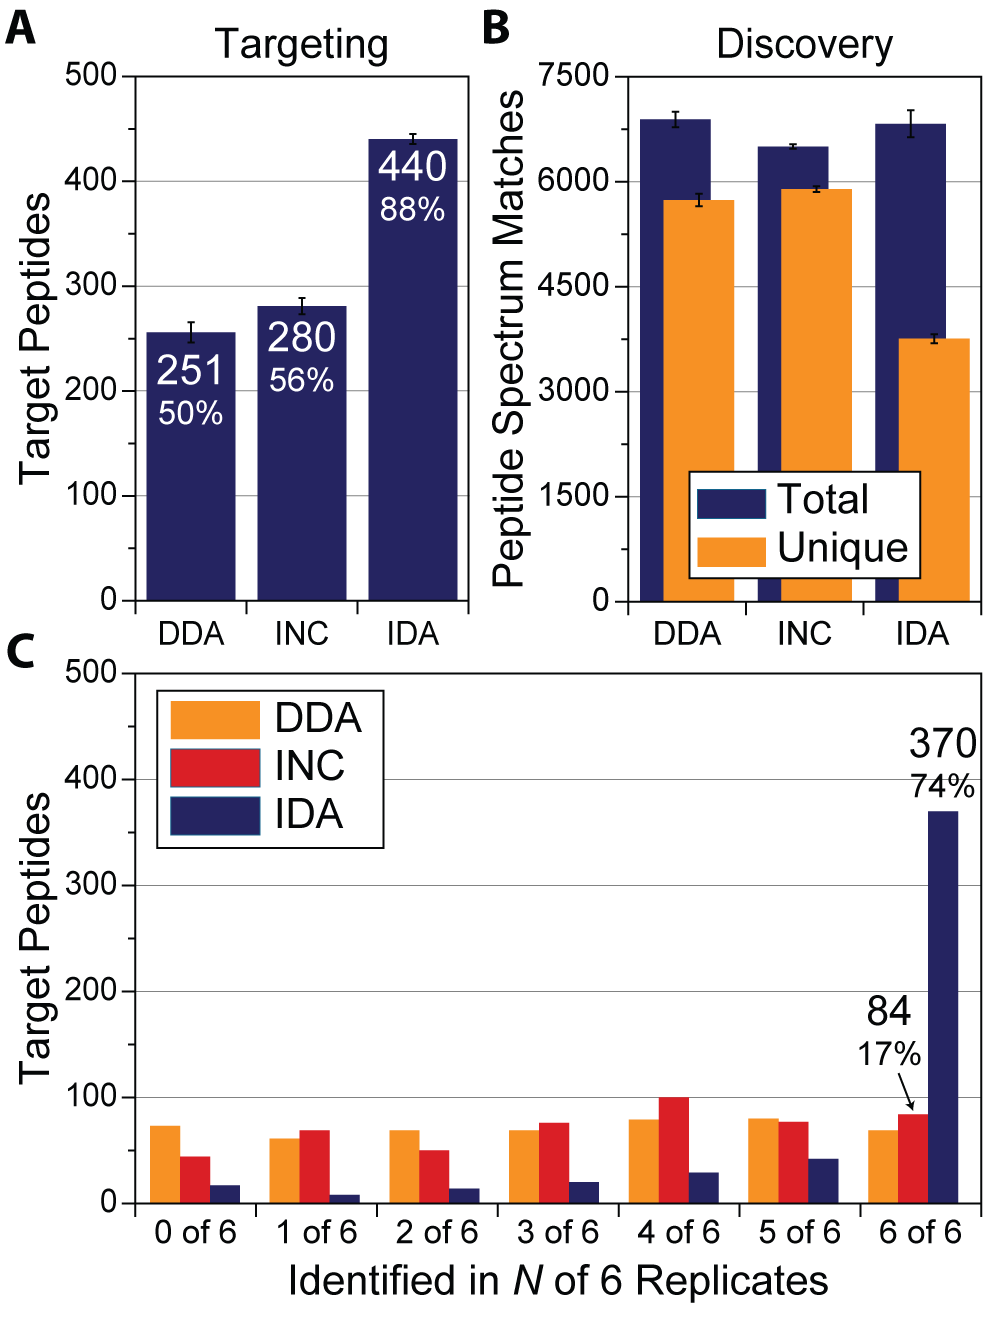
\includegraphics[width=0.75\columnwidth]{eoa/EOA 5.png}
	\mycaption{Reproducibility improvements using intelligent data acquisition}{A subset of 500 mouse peptides were targeted with DDA, an accurate mass inclusion list (INC), and our intelligent data acquisition (IDA) method in hexplicate. (A) IDA identified the most target peptides of the three methods (error bars represent 1 $\sigma$). (B) Discovery identifications by three methods show only a slight decline in the total number of peptides identified using IDA. (C) 74\% of the targets were observed in all six technical replicates when IDA was used compared to less than 20\% for the inclusion list or data dependent acquisition.}
	\label{fig:eoa5}
\end{figure}  
This is consistent with the discovery data where the selected target peptides originated from three of six experiments (50\%). The accurate mass inclusion list modestly increases identifications to 280 (56\%) but the biggest improvement is realized with IDA, where 440 of 500 targets (88\%) were identified on average. Since the IDA method enables simultaneous un-targeted MS/MS sampling, comparisons of the total number of peptide identifications between the three acquisition methods can be made (Figure \ref{fig:eoa5}B). Each method produced nearly the same number of peptide spectral matches (PSMs). A difference appears at the unique PSMs level (i.e., peptides) where both DDA and INC produced similar number of identifications (\textasciitilde5,800 peptides) but dropped to \textasciitilde3,700 using IDA. We attributed this decline primarily to the redundant sampling of target peptides with the IDA method compared to the other methods. IDA identified each target 4.3 times on average, compared to 0.59 and 0.63 for DDA and INC respectively, a \textasciitilde7:1 ratio. This is in agreement with the ratio of dynamic exclusion times between methods; IDA uses 5 seconds for each target, compared to the longer dynamic exclusion time (35 s, 1:7) used in the DDA and INC methods. The oversampling of target peptides in IDA increases the likelihood of identification. We feel that it is an acceptable tradeoff between maximizing reproducibility for a subset of peptides and a slight decline in total identified peptides. The increased reproducibility is demonstrated in Figure 5C; the IDA method identified 370 (74\%) of the same peptides in all six experiments. The same cannot be said for DDA or INC, which only managed to identify 69 and 84 peptides in all six experiments, respectively. This represents an increase of over 340\% in the number of peptide targets that were seen in all replicates.

\subsection*{Improved Reproducibility in Biological Systems.}

All data described above have consisted of technical replicates of the same sample, injected with the same HPLC, and analyzed using the same MS. These technical replicates are ideal to develop acquisitions methods on, primarily because the same peptides should exist in each injection, which removes sample variability from obfuscating the results. However, biological replication in proteomic studies is becoming more prevalent, due to the increase in statistical power it affords. To test whether intelligent data acquisition improves reproducibility in biological systems, four male C57BL/B6 mice were sacrificed at ten weeks, eight organs were harvested, and peptides from a tryptic digestion of each organ was labeled with a TMT 8-plex tag (Figure \ref{fig:eoa6}A\&B).
\begin{figure}[p]
	\centering
	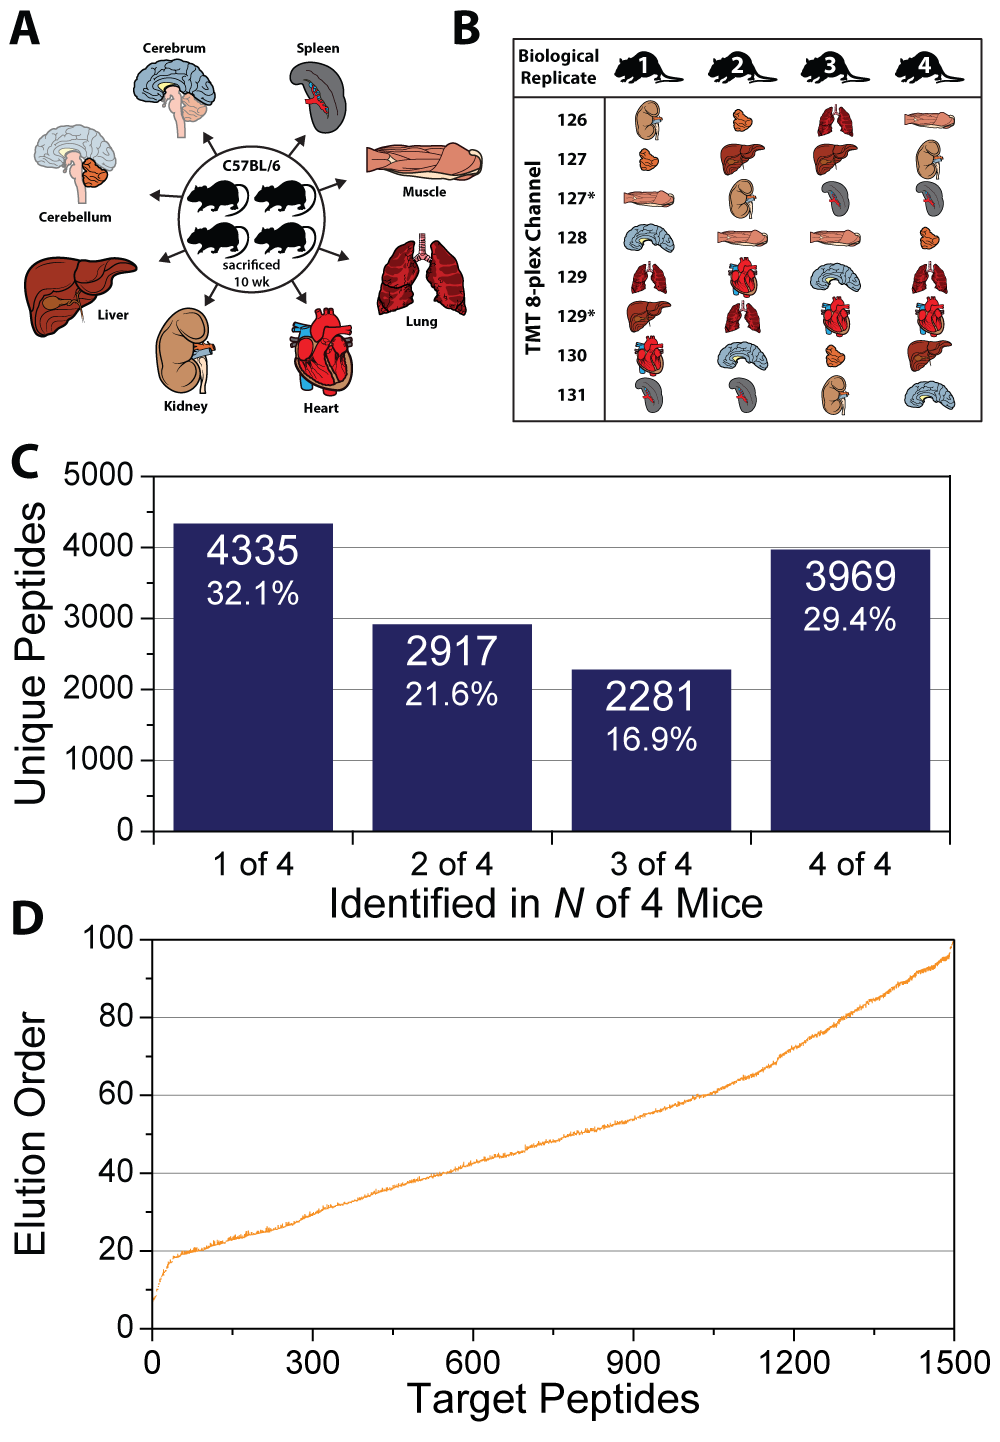
\includegraphics[width=0.75\columnwidth]{eoa/EOA 6.png}
	\mycaption{Peptide targets of biologicial replicates of mice}{(A) Four C57BL/6 mice were sacrificed at 10 weeks of age and eight organs were harvested from each mouse.  (B) Peptides resulting from a tryptic digestion of lysates from each organism were labeled with TMT 8-plex tags in a randomized order (C) 165 minute nano-LC-MS/MS experiments using DDA top-15 method only identified 3,969 peptides in all four mice. (D) A subset of 1,500 peptide targets were selected from peptides only detected in 2 or 3 of all 4 mice.}
	\label{fig:eoa6}
\end{figure}
The tagged peptides from each mouse were mixed together and separated over a 165 minute gradient and sampled using a DDA top-15 method to generate a list of peptide targets. An average of 8,683 $\pm$313 peptide sequences were identified in each mouse for a total of 13,502 unique sequences. Of these, only 3,969 (29.4\%) peptides were identified in every mouse (Figure \ref{fig:eoa6}C). A subset of 1,500 peptides were selected from the peptides detected in either two or three of four mice and sorted based on their assigned elution orders (Figure \ref{fig:eoa6}D). Here, peptide targets were chosen to be evenly distributed in the elution order dimension to limit the number of coeluting peptides at a given point. In subsequent targeting experiments, each mouse sample was analyzed twice, once using DDA and the other IDA, for a total of eight experiments. When the DDA targeting experiments were analyzed, an average of 810 (54\%) target peptides were identified (Figure \ref{fig:eoa7}A, 1\% FDR, error bars represent one $\sigma$). Using IDA, this number increases to 1,072 (71.5\%).

In total, over half of the targeted peptides (826, 55.1\%) were identified in all four mice when using IDA compared to only 30.6\% (459) using DDA (Figure \ref{fig:eoa7}B). The IDA method represents a nearly 80\% improvement over DDA in the number of peptide targets it identifies in all mice. This increase in reproducible identification improves the quantitative results as well. When each tissue is compared to liver, the number of peptides that could be statistically quantified (p-value < 0.05) is on average 227 greater with IDA compared to DDA (Figure \ref{fig:eoa7}C). For example, when the quantitative data for muscle is compared to liver (Figure \ref{fig:eoa7}D), IDA produced 826 significantly different peptides while only 531 were significant for DDA, a 56\% increase. This can be directly attributed to increased reproducibility in identification across biological samples.
\begin{sidewaysfigure}[p]
	\centering
	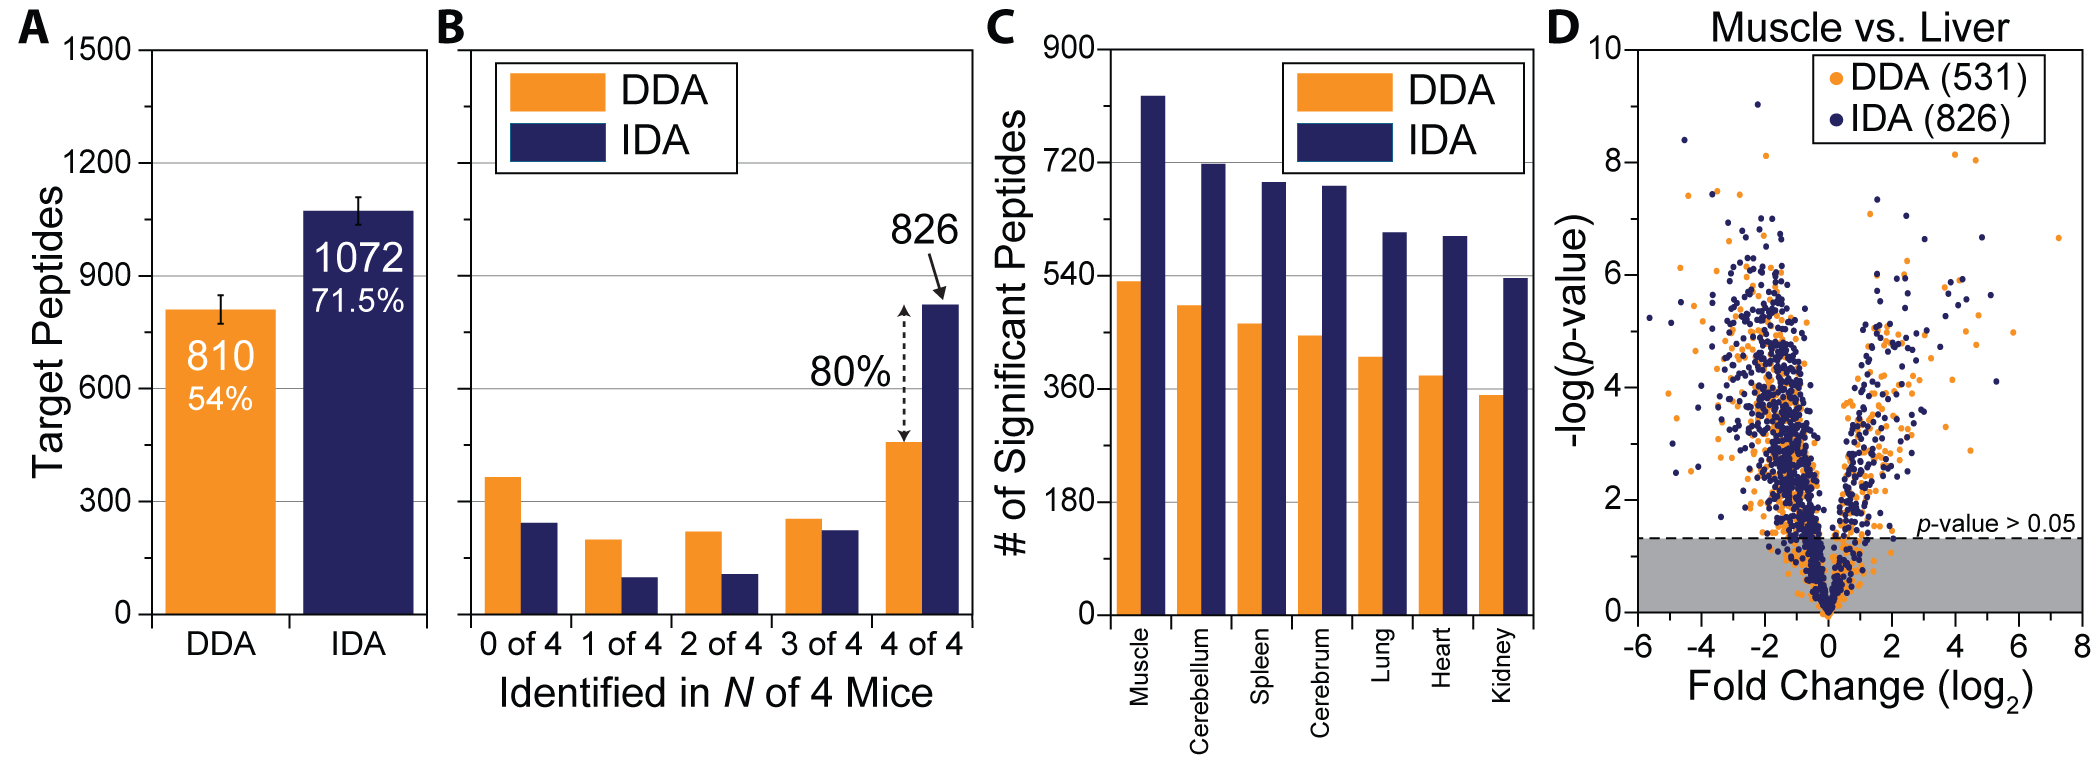
\includegraphics[width=\columnwidth]{eoa/EOA 7.png}
	\mycaption{Identification and quantification improvements in biological replication}{(A) In four subsequent nano-LC-MS/MS experiments, only 810 of 1,500 mouse peptide targets were identified with DDA. The identifications improve to 1,072 when IDA is used (error bars represent 1 σ). (B) In total, 826 target peptides were identified in all four mouse when IDA was used to target. This number falls to only 459 peptides when DDA is used. (C) The number of statistically significant differences (p-value < 0.05) quantified when each tissue is compared to liver is greater with IDA than DDA. (D) When comparing target peptides identified in the muscle vs. the liver, IDA quantified 826 statistically significant peptides compared to only 531 when DDA was used, a 56\% increase.}
	\label{fig:eoa7}
\end{sidewaysfigure}

\section{Conclusion}

The ability to identify the same peptides in multiple experiments reproducibly is increasingly important in proteomic analysis as increased statistical power is demanded. Historically---the most common acquisition method, data-dependent acquisition (DDA) has been used to sample large portions of proteomes, but lacks adequate peptide identification reproducibility. In this manuscript, we expand upon our previous intelligent data acquisition (IDA) work and introduce the concept of using elution order as a way to schedule and target peptides.  Here we have described an online elution order alignment (EOA) algorithm that automatically adjusts to different chromatographic conditions to deliver consistent scheduling and robust reproducibility. The method is capable of targeting large numbers of peptides (>500) in a single run with minimal upfront preparation and effort. Using this method, we have shown great improvements in peptide identification overlap among multiple experiments compared to DDA (88\% compared to 50\% identification overlap in six experiments). The EOA algorithm is capable of improving reproducibility even for highly variable samples. In four mice, our method was able to identify 806 target peptides compared to only 459 using normal DDA sampling. 

We believe that such technologies can now be applied to traditional SRM methods that use triple quadrupole mass spectrometers. Here, periodic full MS scans could be performed and analyzed to calculate the current elution order and adjust the timing of the SRM transitions. One challenge would be the decreased specificity in determining elution order from low resolution scans. However, using a more adaptable metric for scheduling (elution ordering vs. retention time) could potentially increase the portability and robustness of SRM methods while reducing development time. 

A novel aspect of our method is the combination of discovery and targeted analysis in a single method. The MS intelligently switches between targeted and discovery modes depending on what is currently eluting, without any human intervention. In one experiment, over 3,700 unique mouse peptides were discovered using DDA while simultaneously targeting 500 peptides. Such hybrid MS methods enable both a focused and holistic view on the same sample, something that is welcomed when sample-limited. 

Until comprehensive proteomic coverage is routinely obtained, targeted methods will be heavily used and developed. We have explored increasing the intelligence of MS methods as a means to improve the throughput and power of peptide targeting, without sacrificing the novel discovery aspect of DDA sampling. Future work includes improvements to the determination of elution orders, increasing the success rate of target identification, and maximizing the throughput to target larger portions of the proteome without laborious upfront work.

\section{Experimental Methods}

\subsection*{Yeast Culture.}
\emph{Saccharomyces cerevisiae} strain BY4741 was grown in yeast extract peptone dextrose media (YPD) (1\% yeast extract, 2\% peptone, 2\% dextrose). A starter culture was added to 2 L of media and was propagated for \textasciitilde12 generations (20 hours) to a total OD$_{600}$ of \textasciitilde2. The cells were pelleted with centrifugation at 5,000 rpm for 5 min, supernatant decanted, and re-suspended in chilled NanoPure water. Washing with water was repeated twice and the final pelleting was performed at 5,000 rpm for 10 min. The pellet was resuspended in lysis buffer composed of 50 mM Tris pH8, 8 M urea, 75 mM sodium chloride, 100 mM sodium butyrate, protease and phosphatase inhibitor tablet (Roche). Cell lysing was performed with glass bead milling in a stainless steel container (Retsch). A 2.5 mL aliquot of resuspended yeast were shaken with 2 mL of acid-washed glass beads at 30 Hz for 4 min, followed with 1 min rest, for eight cycles.

\subsection*{Mouse Handling and Tissue Isolation.}
Four male C57BL/B6 mice were bred from in-house colonies and housed in an environmentally controlled facility with free access to water and standard rodent chow (Purina \#5008). Mice were kept in accordance to the University of Wisconsin-Madison Research Animals Resource Center and NIH guidelines for care and use of laboratory animals. At 10 weeks of age, mice were sacrificed by decapitation after a four hour fast. Eight tissues were dissected from the mice (cerebellum, cerebrum, kidney, heart, liver, lung, extensor digitorum longus, and spleen), flash frozen in liquid nitrogen and stored at -80$^\circ$C. Tissues were homogenized in 1 mL lysis buffer/100 mg tissue (8 M Urea, 50 mM Tris, 100 mM NaCl, 1 mM CaCl$_2$, 100 mM sodium butyrate, 5 $\mu$M MS-275, 0.2 $\mu$M SAHA, Roche protease and phosphatase inhibitor tablets).

\subsection*{Sample Preparation.}
Protein was quantified by BCA (Pierce) and reduced with 5 mM dithiothreitol and incubated for 45 minutes at 55$^\circ$C. Alkylation was performed with 15 mM iodoacetamide for 30 minutes in the dark and quenched with 5 mM dithiothreitol. Urea concentration was diluted to 1.5 M with 50 mM Tris pH 8.0. Proteolytic digestion was performed by addition of Trypsin (Promega), 1:50 enzyme to protein ratio, and incubated at ambient temperature overnight. For quantitative studies, the resulting peptides were labeled with TMT 8-plex (Pierce) isobaric tag, and mixed.\cite{tmt8,tmt82} All samples were desalted using C-18 solid phase extraction (SPE) columns (Waters, Milford, MA) prior to nano-LC-MS/MS analysis.

\subsection*{Nano LC-MS/MS analysis.}
Peptides were separated with online reverse-phase chromatography using a nanoACQUITY UPLC system (Waters, Milford, MA). Peptides were first loaded onto a precolumn (75 $\mu$m ID, 5 cm Magic C18 particles, Bruker, Michrom) for 10 min at 1 $\mu$l/min flow rates. Peptides were then separated on a 30 cm analytical column (75 $\mu$m ID, 5 cm Magic C18 particles) for either 100 or 160 min over a linear gradient from 8\% to 35\% acetonitrile at 300 nl/min. Mass analysis was performed on an LTQ Orbitrap Elite mass spectrometer (Thermo Fisher Scientific, San Jose, CA) using 60,000 resolving power (RP) MS scans.\cite{orbielite} Peptides selected for MS/MS analysis used a 2 Th isolation width, fragmented with HCD (NCE = 35), and analyzed in the Orbitrap at 15,000 RP or 30,000 RP for quantitative experiments. Unless otherwise noted, data-dependent analysis was performed selecting the top 15 most intense \mz{} features (charge state >1) for MS/MS analysis. Dynamic exclusion settings were enabled for 35 s at $\pm$10 ppm mass window, 1 occurrence with a maximum of 500 exclusions at any given point in time. Automatic Gain Control (AGC) was enabled and MS targets were set to 1\e{6} and MS/MS targets were set to 5\e{4}. Accurate mass inclusion list experiments would prioritize MS/MS sampling from a list of targets at $\pm$10 ppm mass tolerances. Remaining MS/MS events were filled with normal top-N DDA approaches. Intelligent data acquisition control was implemented using the ion trap control language (ITCL, Thermo Fisher Scientific). Briefly, following MS analysis, the spectra was analyzed using algorithms written in ITCL to select targets for MS/MS analysis (described herein). Any remaining MS/MS slots would be filled by the unmodified DDA firmware code.

\subsection*{Data Analysis.}
Thermo .raw files were processed using the Coon OMSSA Proteomic Analysis Software Suite (COMPASS) and in-house software.\cite{compass} Briefly, raw files were converted to the dta file format (DTA Generator) and were searched using the Open Mass Spectrometry Search Algorithm (OMSSA, v 2.1.9).\cite{omssa} Yeast data was searched against a target-decoy database of yeast ORFs (www.yeastgenome.com, February 3, 2011) and mouse data from UniProt canonical database.\cite{targetdecoy} Peptides were generated from a tryptic digestion with up to three missed cleavages, carbamidomethylation of cysteines as fixed modifications, and oxidation of methionines as variable modifications. For quantitative experiments, a fixed modification of 8-plex TMT tag was added to lysines and peptide n-terminus, with a variable modification of 8-plex TMT tag on tyrosines. Precursor mass tolerance was 100 ppm using the multiisotope function (-tem 4 -ti 4) and product ions were searched at 0.015 Da tolerances. Peptide spectral matches (PSM) were validated using FDR Optimizer based on q-values at a 1\% false discovery rate (FDR). Protein groups were constructed from peptide identifications according to the law of parsimony and filtered to a 1\% FDR (Protein Hoarder). For quantitative datasets, peptides were quantified with TagQuant (v1.4) using the generated TMT 8-plex reporter ions, corrected for isotopic impurities, and normalized to total protein abundance. Peptide Elution orders determination algorithms were performed by custom software developed in C\# with the Microsoft .NET Framework version 4.5. 

\bibliographystyle{ieeetr}
\bibliography{eoa}